\documentclass[10pt,a4paper]{article}
\usepackage[margin=20mm,headheight=15pt]{geometry}
\usepackage{amsmath,amssymb,graphicx,booktabs,caption,enumitem,array,fancyhdr}
\usepackage{fontspec}

\setmainfont{Latin Modern Roman}
\usepackage[colorlinks=true,linkcolor=blue,urlcolor=blue,citecolor=blue]{hyperref}
\setlength{\parindent}{0pt}\setlength{\parskip}{5pt}
\setlist{nosep,leftmargin=1.5em,topsep=3pt}
\captionsetup{font=small,labelfont=bf,skip=4pt}
\pagestyle{fancy}\fancyhf{}\fancyhead[L]{ELEN90099 | LDI Preliminary Report}\fancyhead[R]{October 2026}\fancyfoot[C]{\thepage}
\setlength{\emergencystretch}{3em}
\begin{document}\begin{titlepage}\thispagestyle{empty}\centering\vspace*{22mm}
{\Large ELEN90099 Deep Learning\par}\vspace{8mm}
{\LARGE\bfseries Multi-step Electricity Load and Solar Output Forecasting\\[4mm]Initial Experiments, Model Comparisons and Validation Plan\par}\vspace{10mm}
{\large Learn--Design--Implement Project\\Preliminary Report / English Submission Version\par}\vspace{12mm}
Both student names and student IDs: TO BE COMPLETED.\\[3mm]Section authorship: TO BE COMPLETED.
\vspace{12mm}\begin{minipage}{0.88\textwidth}
\textbf{Abstract. }Using fixed 16-channel subsets from original Monash releases, this project compares 48-hour-history to 24-hour-horizon forecasting for electricity load and solar output. All models share chronological splits, training-only scaling and evaluation origins. Initial main experiments use three fixed seeds and a five-epoch ceiling, with single-seed history/data sensitivity studies. The methods span persistence, daily naive, LSTM, GRU, CNN, CNN--LSTM, a self-written DLinear and a simplified PatchTST-style model. The patch model merits further Electricity validation, whereas daily naive remains stronger on Solar under this budget. Saved predictions, checkpoints and SQLite records support result verification. The report distinguishes observed accuracy and local GPU costs from untested deployment implications, and gives a concrete final-report plan.
\end{minipage}\vfill
Nine body pages; title and references excluded from the preliminary page count.\\Author fields intentionally remain incomplete pending confirmation.
\end{titlepage}\setcounter{page}{1}
\section{Introduction, scope and literature}
\noindent\textit{Section author: to be completed.}


\subsection{Engineering problem and motivation}
Day-ahead electricity demand and photovoltaic (PV) output forecasts can inform scheduling and storage decisions. Here the engineering objective is narrower: predict the next 24 hours using only the preceding 48 hours of observed target values, and assess whether added model complexity improves accuracy enough to justify its computational cost. Forecasting is studied as a supervised sequence-to-sequence regression problem, not as an operational dispatch controller. No claim about realised cost savings, grid safety or deployment is made.

The study uses two separate energy tasks: hourly Electricity and ten-minute Solar from the Monash archive~\cite{monash,electricity,solar}. Each task has 16 fixed, aligned channels and its own independently trained models. Weather, calendar features, future observations and other datasets are excluded. This limited information set makes comparisons clear, but also limits the ability to anticipate weather-driven changes in PV generation. The Solar release has a simulated source; using an original benchmark file does not make it a field deployment dataset~\cite{solar}.
\subsection{Research questions and measurable outcomes}
\begin{enumerate}
\item Do trainable models improve on persistence and a daily seasonal naive predictor on the same forecast origins?
\item How do recurrent memory, local convolution, hybrid encoding, linear decomposition and patch attention differ in accuracy and resource use?
\item Does the ranking change with forecast distance, high-load/active-output conditions, history length or available training data?
\end{enumerate}
Success is assessed by original-scale MAE and RMSE, channel-averaged seasonal MASE, and measured training/inference costs. Beating a strong daily baseline is more informative than beating persistence alone. A negative result is useful when the comparison protocol and its limits are explicit.
\subsection{Related methods and course connections}
LSTM~\cite{lstm} and GRU~\cite{gru} provide gated recurrent state updates; a temporal CNN tests local filters and weight sharing. Their comparison links recurrence, gradient-based learning and convolution to the course. CNN--LSTM tests a serial composition, while leaving open whether extra capacity rather than complementary mechanisms explains any improvement. DLinear~\cite{dlinear} challenges the assumption that nonlinear attention is necessary. PatchTST~\cite{patch} motivates patches and channel-shared encoding, giving a different temporal representation.

The implementation uses self-written PyTorch classes. In particular, the attention model is called \emph{PatchTST-style}: it preserves patching and channel independence but is not an exact reproduction of the published model or a direct import from Time-Series-Library. This report evaluates the supplied implementation, not a published benchmark ranking.
\subsection{Preliminary status and report structure}
This preliminary submission contains three-seed, five-epoch-budget main comparisons and single-seed sensitivity experiments on original releases. Sections 2--5 define the data, protocol, designs and implementation; Sections 6--8 report initial findings; Section 9 gives limitations, final-report tasks and conclusions. The complete final-report structure is therefore visible even where further validation remains planned~\cite{course}.

\clearpage
\section{Data provenance and exploratory analysis}
\noindent\textit{Section author: to be completed.}


\subsection{Release checks and frozen subset}
The downloaded ZIP and extracted TSF files are checksummed. Every source series is checked for finite values, common length/start time, and nonconstant training data. The selected IDs are matched by \texttt{series\_name}, never by an assumed zero-based numeric position. No interpolation or unit conversion is applied; quantities are reported in original release units because their physical interpretation has not been independently resolved for these aggregate files.
\begin{center}\small
\begin{tabular}{lrr}\toprule
Property & Electricity & Solar\\\midrule
Source series / selected & 321 / 16 & 137 / 16\\
Samples per series & 26,304 & 52,560\\
Sampling / daily period & 1 hour / 24 & 10 minutes / 144\\
Source start & 2012-01-01 00:00:01 & 2006-01-01 00:00:01\\
History / horizon (steps) & 48 / 24 & 288 / 144\\
Training zero values & 0.0\% & 53.0\%\\
\bottomrule\end{tabular}\end{center}

Subset selection uses only the first 70\% of each source: stable sorting by mean, four rank groups, and four random draws per group with a newly initialised NumPy RNG (seed 42) for each dataset. The selection is independently reproduced and matches the frozen outline IDs. This stratifies average scale; it does not establish population representativeness.
\begin{quote}\small
Electricity: T5, T8, T21, T30, T99, T133, T144, T146, T198, T219, T231, T251, T285, T291, T304, T309.\\
Solar: T7, T9, T27, T28, T41, T58, T60, T64, T69, T77, T82, T97, T115, T123, T127, T131.
\end{quote}
\begin{center}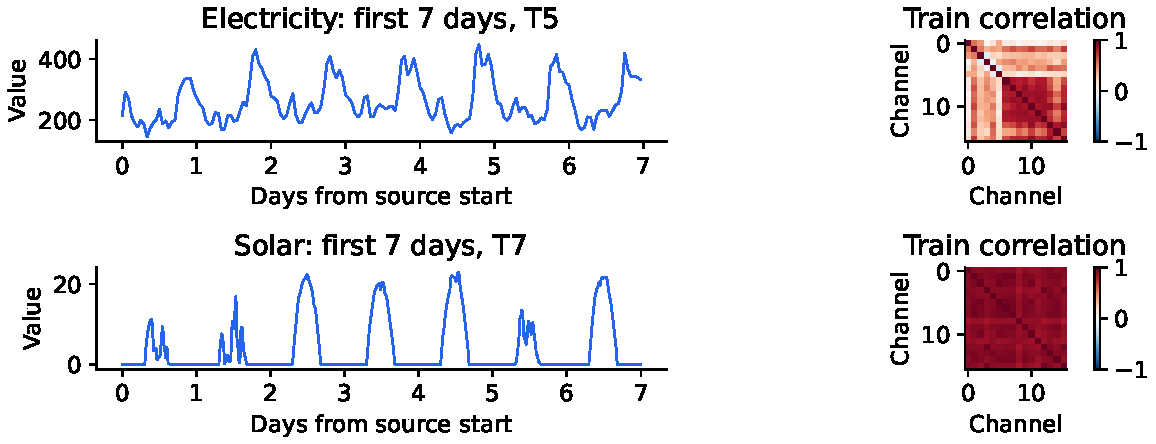
\includegraphics[width=\textwidth,height=6.1cm,keepaspectratio]{figures/data_overview.pdf}\captionof{figure}{Fixed first-channel profiles and training-only correlation. The first seven source days are displayed without selecting an attractive forecast.}\end{center}
\subsection{Implications for model design}
The raw profiles and training correlations motivate daily baselines and both channel-mixing and channel-independent designs. Correlation alone does not prove a causal interaction or that cross-channel attention is needed. High solar zero prevalence can lower overall error while concealing errors during output activity; both full and conditional metrics are retained. Different users/plants have different scales, motivating per-channel normalisation and a scaled metric alongside absolute errors. The implicit source time grid is retained without assigning an unverified local timezone or interpreting clock hours as confirmed sunrise/sunset.

\clearpage
\section{Forecasting formulation and evaluation protocol}
\noindent\textit{Section author: to be completed.}


\subsection{Information available at each origin}
Let $X\in\mathbb R^{T\times C}$, $C=16$. At origin $t$, the input is $X_{t-L:t}$, using half-open slices, and the label is $Y_t=X_{t:t+H}$. Every model returns all $H\times C$ targets in one pass. Electricity uses $(L,H)=(48,24)$; Solar uses $(288,144)$. No target within $[t,t+H)$ enters the input. Later rolling origins may use observations revealed since earlier origins; this is rolling-origin forecasting rather than a single frozen forecast made at the beginning of the test interval.
\subsection{Chronological partition and standardisation}
Set $b_1=\lfloor0.70T\rfloor$ and $b_2=\lfloor0.80T\rfloor$. Training targets lie within $[0,b_1)$, validation within $[b_1,b_2)$, and test within $[b_2,T)$. A complete target must fit inside its own interval. Historical context may extend into an earlier split because it is already observed. Training origins advance by three hours; validation/test origins by one hour. Shuffling is limited to the already isolated training windows.
\begin{center}\small
\begin{tabular}{lrrrrr}\toprule
Dataset & $b_1$ & $b_2$ & Train origins & Val origins & Test origins\\\midrule
Electricity & 18412 & 21043 & 6114 & 2608 & 5238\\
Solar & 36792 & 42048 & 2021 & 853 & 1729\\
\bottomrule\end{tabular}\end{center}

Each channel is standardised using only the available training interval: $z_{tc}=(x_{tc}-\mu_c)/\max(\sigma_c,10^{-8})$. Validation/test use the same statistics, and predictions are inverse transformed before reporting errors. Standardised MSE is used for fitting and validation selection. It gives a different channel weighting from raw-scale MAE; the distinction matters for interpreting rankings.
\subsection{Metrics and aggregation}
For $N$ origins, horizon $H$, channels $C$, and errors $e_{thc}=\hat y_{thc}-y_{thc}$,
\begin{align}
\mathrm{MAE}&=\frac1{NHC}\sum_{t,h,c}|e_{thc}|,&
\mathrm{RMSE}&=\sqrt{\frac1{NHC}\sum_{t,h,c}e_{thc}^2},\\
q_c&=\frac1{T_{\rm tr}-m}\sum_{s=m}^{T_{\rm tr}-1}|x_{sc}-x_{s-m,c}|,&
\mathrm{MASE}&=\frac1C\sum_c\frac{\mathrm{MAE}_c}{\max(q_c,10^{-8})}.
\end{align}
Here $m$ is one day and $q_c$ uses only that run's training interval~\cite{mase}. The global RMSE is not an average of channel RMSEs. MASE below one compares against in-training seasonal differences; it does not automatically imply beating the seasonal naive model on the test interval. MAE/RMSE from the two datasets must not be numerically ranked against each other.
\subsection{Forecast distance, conditional slices and dependence}
Report both the first four hours and the full 24 hours, plus each lead time in hours. The Electricity peak mask is true output at or above the channel's training 85th percentile. The Solar active mask is true output at or above 10\% of its training maximum. These are post-hoc evaluation masks, not inputs; active output is not a verified astronomical daytime label. Raw negative predictions remain in all main scores.

Hourly rolling windows overlap substantially. Their errors are dependent, so the number of windows is not an independent sample size. Seed standard deviations describe training variability only; no independent-window significance test is reported.

\clearpage
\section{Model mechanisms and design choices}
\noindent\textit{Section author: to be completed.}


\subsection{Two non-learning controls}
Persistence sets $\hat y_{t+h,c}=x_{t-1,c}$. Daily naive repeats the latest observed day, $\hat y_{t+h,c}=x_{t+h-m,c}$ for $h=0,\ldots,H-1$, where $H=m$. Both see only the same history as trainable models. They have no fitted parameters and test whether continuity or diurnal repetition already explains most predictable variation.
\subsection{Recurrent and convolutional networks}
The one-layer LSTM has hidden size 64 and updates its memory using
\[
c_s=f_s\odot c_{s-1}+i_s\odot\tanh(W_g[x_s,h_{s-1}]+b_g),\qquad h_s=o_s\odot\tanh(c_s),
\]
where $i_s,f_s,o_s$ are sigmoid gates~\cite{lstm}. The final hidden state is linearly projected to $HC$ outputs. Gating provides a learnable memory path; it does not guarantee that a short training budget learns a full weekly dependency. GRU uses update/reset gates and a single hidden state~\cite{gru}, reducing recurrent parameters. Both mix the 16 inputs at each time step and compress the history into a final state.

The 1D-CNN applies temporal kernels of width three, channels $16\to32\to64$, batch normalisation and ReLU, followed by adaptive average pooling to 16 positions and a dense $HC$ head. Its two convolutions have a five-step local receptive field before pooling. Pooling aggregates local features over the complete history; this is not a dilated temporal convolutional network and not proof of explicit long-range interaction. Symmetric convolution padding uses only the observed history, so it does not expose future targets.
\subsection{Hybrid CNN--LSTM}
The hybrid applies a $16\to64$ width-three convolution with batch normalisation/ReLU, then a 64-unit LSTM and direct dense head. The hypothesis is that local features simplify recurrent encoding. Comparing it with LSTM is a useful architecture comparison, but not an isolated causal ablation: its input representation and parameter count also change. Capacity-matched and frontend-removal controls remain final-report work.
\subsection{Decomposition and patch attention}
DLinear decomposes the history into an endpoint-replicated 25-step moving average $T$ and remainder $R=X-T$, and predicts
\[\hat Y_{c,:}=W_TT_{c,:}+W_RR_{c,:}+b_T+b_R.\]
The two maps are shared across channels and contain $2H(L+1)$ parameters. The remainder is not guaranteed to be a pure physical seasonal component. A 25-step smoother spans 25 hours on Electricity but only 4 h 10 min on Solar, so equal step settings are not equal physical filters~\cite{dlinear}.

The PatchTST-style model independently patches each channel (length 16, stride 8), projects patches to width 64, adds learnable positions, applies two Transformer encoder layers (four heads, feed-forward width 128, dropout 0.1), and flattens tokens to an $H$-output head. The scaled dot-product attention operation is $\mathrm{softmax}(QK^\top/\sqrt{d_k})V$~\cite{patch}. Channels share weights after folding into the batch dimension; there is no explicit cross-channel attention. With aligned core windows, patch counts are 5 and 35, respectively. Patches span 16 hours versus 2 h 40 min, another frequency-dependent design difference.

This custom attention implementation uses PyTorch LayerNorm encoder blocks, learnable zero-initialised positions, and global training-set scaling without RevIN. It is therefore a simplified implementation inspired by PatchTST, not an exact upstream reproduction. DLinear also uses the local class's random initialisation. These choices are recorded rather than attributing the observations to all versions of the original models.

\clearpage
\section{Implementation, training and reproducibility}
\noindent\textit{Section author: to be completed.}


\subsection{Initial experiment budget and validation selection}
The preliminary budget is fixed at five maximum epochs, patience three, batch size 32, Adam with learning rate $10^{-3}$ and weight decay $10^{-4}$. No model-specific test-driven search is performed. Main trainable comparisons use seeds 42, 43 and 44; each sensitivity setting uses seed 42. This is a deliberately limited pilot, not a claim of convergence. The final plan extends the maximum to 20 epochs with validation-based choices.

Each epoch visits the complete training-origin set. Validation MSE is summed over all target elements and divided by their count, so a smaller final batch is weighted correctly. The lowest validation-loss state is retained; test metrics are computed from that state even when it is not the final epoch. Identical epoch limits do not equalise parameter counts, FLOPs, optimiser steps across data fractions, or wall-clock budgets. These differences are logged rather than hidden.
\subsection{Measured environment and resources}
All new runs use NVIDIA GeForce RTX 3060 Laptop GPU, PyTorch 2.5.1+cu121, Python 3.10.21 and NumPy 2.2.6. 
This is a local GPU experiment, not measured Colab T4 performance. The same code can be run in Colab; elapsed times must be measured again there.

Training time includes the epoch loop and validation. Peak allocated CUDA memory is recorded for the training phase. Inference measures a model-only forward pass with the input already resident on the device, after ten warmups and 30 synchronised wall-clock repetitions. It excludes loading, host-device transfers, standardisation and database/file writes; it is not an end-to-end deployment SLA. The resource summary below averages training times and per-run median latencies over main seeds.\par
\begin{center}\small
\begin{tabular}{lrrrr}\toprule
Model & Params E & Params S & Train s E / S & Median ms E / S\\\midrule
LSTM & 45,952 & 170,752 & 8.2 / 1.4 & 0.38 / 0.66\\
GRU & 40,704 & 165,504 & 3.4 / 1.3 & 0.41 / 0.50\\
1D-CNN & 401,568 & 2,369,568 & 4.3 / 1.7 & 0.72 / 0.77\\
CNN-LSTM & 61,504 & 186,304 & 4.5 / 1.7 & 0.98 / 1.00\\
DLinear & 2,352 & 83,232 & 3.0 / 1.2 & 0.52 / 0.52\\
PatchTST-style & 76,056 & 392,976 & 9.4 / 5.2 & 1.52 / 3.47\\
\bottomrule\end{tabular}\end{center}

\subsection{What the code package records}
\texttt{prepare\_data.py} obtains original releases and saves hashes/IDs; \texttt{data\_loader.py} enforces verified provenance and split rules. \texttt{experiment.py} trains and evaluates every model through one interface. Unique run directories hold the best checkpoint, scaler, split origins and all test predictions. JSON records and the SQLite \texttt{runs} table retain hyperparameters, losses, epochs, optimiser steps, environment, metrics and relative artifact paths. SQLite satisfies database storage; vector retrieval is not implemented or claimed.

\texttt{verify\_results.py --reload} recomputes errors from saved predictions, checks source alignment and database consistency, and reloads each checkpoint on CPU for a sampled forecast comparison. Contract tests cover leakage boundaries, provenance failures, metrics, forward/backward passes and channel strategy. Successful software tests establish implementation checks, not forecast generalisation. The README documents reconstruction, rerunning, analysis and report compilation.

\clearpage
\section{Initial results and comparative analysis}
\noindent\textit{Section author: to be completed.}


The tables report mean $\pm$ sample standard deviation over seeds 42, 43 and 44 on the same test origins. Deterministic baselines have identical repeated predictions and effectively zero seed deviation; their three records are not three independent forecasting trials. All errors use original release scale except dimensionless MASE. Tables and figures are generated from the new run records, not the legacy database.
\subsection{Electricity: daily structure is a strong control}
\begin{center}\small
\begin{tabular}{lrrr}\toprule
Model & MAE & RMSE & MASE\\\midrule
Persistence & 1,010.261 $\pm$ 0.000 & 3,091.327 $\pm$ 0.000 & 3.630 $\pm$ 0.000\\
Daily naive & 208.218 $\pm$ 0.000 & 732.211 $\pm$ 0.000 & 1.009 $\pm$ 0.000\\
LSTM & 262.727 $\pm$ 4.543 & 727.287 $\pm$ 15.818 & 1.310 $\pm$ 0.015\\
GRU & 262.592 $\pm$ 0.622 & 729.598 $\pm$ 2.779 & 1.304 $\pm$ 0.004\\
1D-CNN & 254.754 $\pm$ 1.493 & 696.794 $\pm$ 17.507 & 1.248 $\pm$ 0.026\\
CNN-LSTM & 267.183 $\pm$ 2.918 & 749.218 $\pm$ 9.099 & 1.310 $\pm$ 0.009\\
DLinear & 220.049 $\pm$ 0.504 & 665.572 $\pm$ 0.484 & 1.032 $\pm$ 0.003\\
PatchTST-style & 203.137 $\pm$ 3.301 & 636.246 $\pm$ 6.630 & 0.959 $\pm$ 0.012\\
\bottomrule\end{tabular}\end{center}
The PatchTST-style model has mean seasonal MASE 0.959, compared with 1.009 for daily naive: an observed 5.0\% reduction. 
The result supports further study of patch-based temporal encoding on this subset, not a general superiority claim. Large raw-scale channels can dominate MAE/RMSE while channel-scaled MASE rewards relative improvement across channels. The comparison should therefore retain all three metrics. Recurrent or hybrid underperformance after five epochs may reflect optimisation, representation bottlenecks or the information set, rather than proving those model families unsuitable.
\subsection{Solar: learn the daily baseline before adding complexity}
\begin{center}\small
\begin{tabular}{lrrr}\toprule
Model & MAE & RMSE & MASE\\\midrule
Persistence & 7.379 $\pm$ 0.000 & 12.546 $\pm$ 0.000 & 3.048 $\pm$ 0.000\\
Daily naive & 2.198 $\pm$ 0.000 & 5.712 $\pm$ 0.000 & 0.900 $\pm$ 0.000\\
LSTM & 3.653 $\pm$ 0.079 & 6.169 $\pm$ 0.192 & 1.493 $\pm$ 0.033\\
GRU & 3.665 $\pm$ 0.131 & 6.126 $\pm$ 0.175 & 1.498 $\pm$ 0.055\\
1D-CNN & 3.020 $\pm$ 0.045 & 4.888 $\pm$ 0.056 & 1.231 $\pm$ 0.018\\
CNN-LSTM & 3.462 $\pm$ 0.082 & 5.930 $\pm$ 0.146 & 1.414 $\pm$ 0.034\\
DLinear & 3.177 $\pm$ 0.037 & 5.236 $\pm$ 0.017 & 1.298 $\pm$ 0.015\\
PatchTST-style & 3.062 $\pm$ 0.036 & 5.100 $\pm$ 0.058 & 1.249 $\pm$ 0.015\\
\bottomrule\end{tabular}\end{center}
Daily naive has mean MASE 0.900; the PatchTST-style model is 38.9\% higher. 
A strong daily baseline is consistent with repeated output profiles, but does not establish that clouds are predictable or that neural models cannot improve with adequate validation-based training. A linear or attention model may smooth sharp output peaks; a recurrent final-state bottleneck also faces a much larger 144-step output. The experiment contains no weather covariates to anticipate genuinely novel cloud conditions.
\begin{center}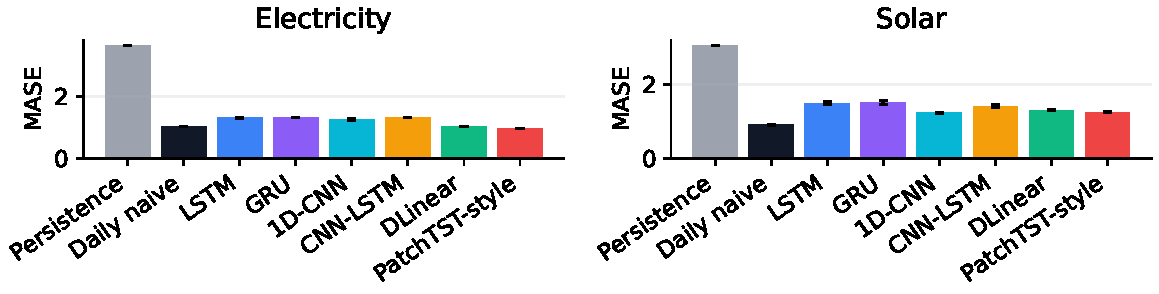
\includegraphics[width=\textwidth,height=3.7cm,keepaspectratio]{figures/comparison.pdf}\captionof{figure}{Initial main comparisons; error bars show training-seed variability, not confidence intervals over independent test days.}\end{center}
\clearpage
\section{Horizon, conditional errors and difficult cases}
\noindent\textit{Section author: to be completed.}


\subsection{Lead time should be read in physical hours}
\begin{center}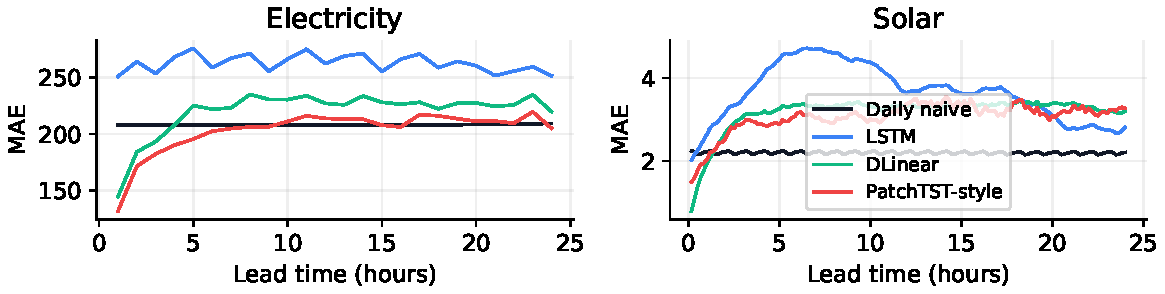
\includegraphics[width=\textwidth,height=4.3cm,keepaspectratio]{figures/lead_time.pdf}\captionof{figure}{Mean per-lead MAE across main seeds; persistence omitted for legibility. Solar steps are ten minutes; Electricity steps are one hour.}\end{center}
Direct multi-output models do not recursively feed their own predictions back. Their lead-time errors may still vary because each output has a different relation to the input and because predictable daily structure reappears. A nonmonotonic curve is therefore possible; monotonically growing error should not be assumed. Persistence loses the benefit of phase alignment, whereas daily naive directly preserves it. These curves describe this rolling-origin evaluation, not an independent error-growth experiment.
\begin{center}\small
\begin{tabular}{lrrr}\toprule
Dataset & Model & First 4h MAE & Conditional MAE\\\midrule
Electricity & Daily naive & 208.122 & 401.885\\
 & LSTM & 259.245 & 461.200\\
 & DLinear & 182.470 & 409.421\\
 & PatchTST-style & 168.821 & 406.685\\
Solar & Daily naive & 2.202 & 5.655\\
 & LSTM & 3.112 & 5.256\\
 & DLinear & 2.463 & 4.896\\
 & PatchTST-style & 2.476 & 4.871\\
\bottomrule\end{tabular}\end{center}

The conditional column uses the training-defined high-load mask for Electricity and active-output mask for Solar. The masks are identical across models within a dataset/configuration. Conditioning can change the mix of channels and magnitudes as well as difficulty; a higher conditional MAE is not alone evidence of a distinct physical failure mechanism. Mask prevalence is saved in the run records.
\subsection{A fixed hard-case rule, including imperfect forecasts}
\begin{center}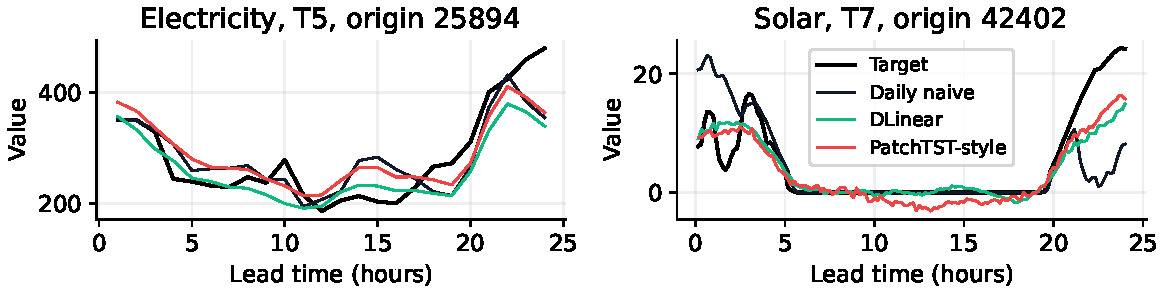
\includegraphics[width=\textwidth,height=4.0cm,keepaspectratio]{figures/hard_cases.pdf}\captionof{figure}{For the first frozen channel, select the origin containing the largest true test target; ties use the earliest origin. The rule never selects by a model error. Seed 42 is fixed, not chosen as the best seed.}\end{center}
These selected peak-output cases expose amplitude and phase mismatches that averaged errors can hide. They are stress illustrations rather than representative or independent evidence. Negative raw outputs are retained in the scores; universal nonnegative clipping can be assessed later as a separate post-processing comparison. The supplied case-selection JSON records the channel and source index so the plots are reproducible.

\clearpage
\section{History and training-data sensitivity}
\noindent\textit{Section author: to be completed.}


\subsection{Controlled design}
Two complementary experiments compare LSTM and PatchTST-style with seed 42 and the same five-epoch ceiling. History lengths are 24, 48 and 168 hours: Electricity lengths 24/48/168; Solar 144/288/1008. All lengths share the training origins admissible under the maximum length, and the same validation/test origins. Thus the 48-hour sensitivity run is retrained on a different common training-origin set than the main comparison; it is not replaced with the main score.

For data amount, use the latest 25\%, 50\% and 100\% of the original training interval, always ending at $b_1$. Both input and target stay within the retained training segment. Each fraction refits its own training-only scaler; fixed channel IDs and validation/test regions do not change. Model selection remains validation-based. The 100\% data setting is rerun rather than borrowed from a different budget.
\begin{center}\small
\begin{tabular}{lrrrrr}\toprule
Dataset & Factor & Model & Small & Middle & Large\\\midrule
Electricity & History & LSTM & 1.319 & 1.319 & 1.318\\
 &  & PatchTST-style & 1.019 & 0.965 & 0.841\\
 & Data & LSTM & 1.428 & 1.350 & 1.304\\
 &  & PatchTST-style & 0.968 & 0.977 & 0.946\\
Solar & History & LSTM & 1.550 & 1.489 & 1.499\\
 &  & PatchTST-style & 1.222 & 1.208 & 1.298\\
 & Data & LSTM & 2.692 & 2.636 & 1.531\\
 &  & PatchTST-style & 1.492 & 1.571 & 1.267\\
\bottomrule\end{tabular}\end{center}

\noindent\small History columns: 24/48/168 hours. Data columns: 25/50/100\%. Values are seasonal MASE.\normalsize
\begin{center}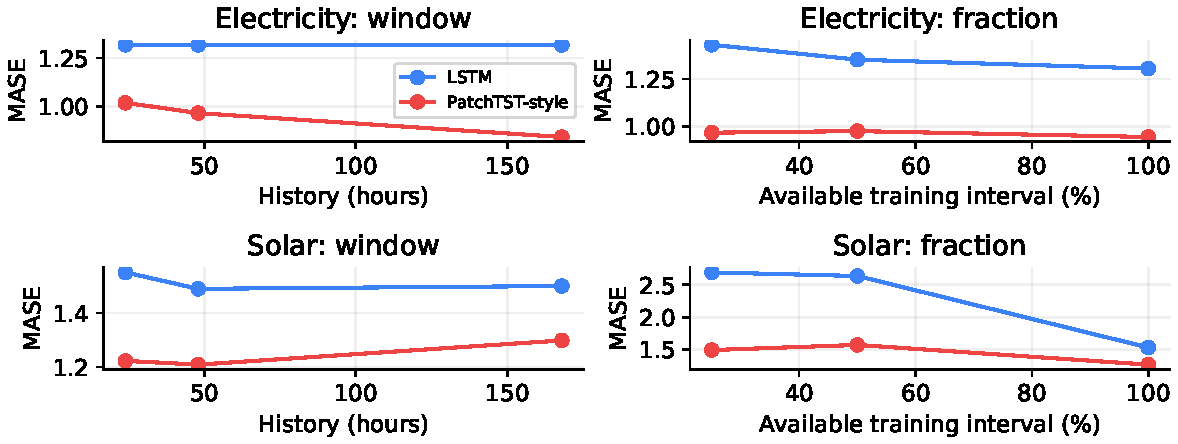
\includegraphics[width=\textwidth,height=5.7cm,keepaspectratio]{figures/sensitivity.pdf}\captionof{figure}{Single-seed controlled sensitivity; lines connect tested settings and do not imply interpolated performance or statistical significance.}\end{center}
\subsection{What can and cannot be inferred}
For Electricity, PatchTST-style changes from MASE 1.019 to 0.841 between the smallest and largest setting. For Solar, LSTM changes from MASE 1.550 to 1.499 between the smallest and largest setting. For Electricity, LSTM changes from MASE 1.428 to 1.304 between the smallest and largest setting.
 These endpoint comparisons do not establish monotonic benefit; the middle setting must also be read. Longer history changes PatchTST-style patch count and dense-head capacity, and changes computation even when recurrent parameter count stays constant. It is therefore a history-plus-capacity sensitivity, not an isolated memory mechanism test.

The fraction experiment changes season coverage, data recency composition and the number of optimiser updates within five epochs. Its MASE denominator is also recomputed on each available segment, so cross-fraction MASE changes can reflect both forecast errors and the reference scale. Use original-scale MAE/RMSE alongside MASE (stored in each JSON), and do not attribute all differences to sample count alone. Multiseed repetitions and a fixed-update-budget comparison remain final-report tasks.

\clearpage
\section{Engineering judgement, limitations and final-report plan}
\noindent\textit{Section author: to be completed.}


\subsection{A provisional engineering choice}
The relevant choice is an accuracy--cost trade-off on each task, not a single architecture winner. On Electricity, compare the PatchTST-style gain with a zero-parameter daily baseline and DLinear's compact maps. On Solar, daily naive is a strong current reference and a sensible fallback under this restricted information set. A more complex model should earn its additional cost through validation that matters for the application, such as peak or active-output errors. None of these initial error reductions is converted into monetary savings or storage control benefit.

Parameter count measures stored weights, while peak memory also includes activations/workspaces. Neither alone measures embedded feasibility: operators, numerical precision, runtime support and end-to-end latency must be checked on the actual target. The observed laptop GPU timings do not support a T4 throughput claim or a microcontroller deployment claim. A Pareto judgement is conditional on chosen objectives and these measurements, not a universal optimum.
\subsection{Limits that affect interpretation}
\begin{enumerate}
\item \textbf{Scope:} the 16 selected channels and one chronological test interval do not establish generalisation to all users/plants, another year, or another region. Solar has a simulated source and no verified astronomical/timezone labels.
\item \textbf{Training:} five epochs and fixed common settings provide a pilot, not equally optimised architectures. Three seeds measure random-initialisation/training variability, not all sources of uncertainty. Some validation curves still improve at the budget limit.
\item \textbf{Mechanisms:} architecture comparisons are confounded by capacity, physical filter span, normalisation and input representation. The self-written PatchTST-style class is not an exact published implementation; pretrained/foundation models and external regressors are outside current scope.
\item \textbf{Evaluation:} overlapping windows and repeated targets induce dependence. Training-scaled MASE, raw MAE/RMSE and conditional slices answer different weighting questions. The test period was already examined in earlier project iterations, so it is not an untouched external blind holdout. New settings were fixed rather than selected by test ranking.
\end{enumerate}
\subsection{Concrete path to the final report}
\begin{enumerate}
\item \textbf{Validation and budget:} inspect losses, extend the ceiling to 20 epochs, and permit a small, documented validation-only search. Record all attempted configurations and equalise the tuning budget; never select the best test seed.
\item \textbf{Sensitivity and ablation:} repeat each sensitivity setting across seeds, report MAE/RMSE as well as MASE, match update budgets as an additional control, and add a capacity-matched CNN frontend comparison. Retain the frozen channel subset and common origins.
\item \textbf{Error analysis:} add channel-level results, weekday/weekend analysis only after timestamp semantics are checked, more predefined hard scenes, residual dependence, and a uniform clipping comparison. If statistical inference is needed, use time blocks rather than treating overlapping windows as independent.
\item \textbf{Deliverables:} confirm authors and section responsibility, polish the final narrative within its separate 20-page total limit, retain the code/database evidence, and prepare the course Q\&A and at-most-three-minute video~\cite{course}.
\end{enumerate}
\subsection{Preliminary conclusion}
The verified experiment shows why baseline strength and protocol correctness precede model complexity. Patch-based encoding merits further Electricity validation, while Solar exposes a substantial gap to the daily control under the pilot budget. The contribution at this stage is a reproducible, comparable set of initial results, an explicit account of model mechanisms, and a controlled plan to test whether the observed trade-offs survive fuller training and broader validation.
\clearpage
\begin{thebibliography}{9}\small
\bibitem{monash} R. Godahewa et al., ``Monash Time Series Forecasting Archive,'' NeurIPS Datasets and Benchmarks, 2021. \url{https://arxiv.org/abs/2105.06643}.
\bibitem{electricity} R. Godahewa et al., Electricity Dataset (Hourly Observations), Zenodo, record 4656140. \url{https://doi.org/10.5281/zenodo.4656140}.
\bibitem{solar} R. Godahewa et al., Solar Dataset (10 Minutes Observations), Zenodo, record 4656144. \url{https://doi.org/10.5281/zenodo.4656144}.
\bibitem{lstm} S. Hochreiter and J. Schmidhuber, ``Long Short-Term Memory,'' Neural Computation, 9(8), 1735--1780, 1997. \url{https://www.bioinf.jku.at/publications/older/2604.pdf}.
\bibitem{gru} K. Cho et al., ``Learning Phrase Representations using RNN Encoder-Decoder for Statistical Machine Translation,'' EMNLP, 2014. \url{https://arxiv.org/abs/1406.1078}.
\bibitem{dlinear} A. Zeng et al., ``Are Transformers Effective for Time Series Forecasting?'' AAAI, 2023. \url{https://arxiv.org/abs/2205.13504}.
\bibitem{patch} Y. Nie et al., ``A Time Series is Worth 64 Words: Long-term Forecasting with Transformers,'' ICLR, 2023. \url{https://arxiv.org/abs/2211.14730}.
\bibitem{mase} R. J. Hyndman and A. B. Koehler, ``Another Look at Measures of Forecast Accuracy,'' International Journal of Forecasting, 22(4), 679--688, 2006. \url{https://robjhyndman.com/papers/mase.pdf}.
\bibitem{course} ELEN90099 teaching team, LDI Project Manual v1, Project Options v1, Inspiration Project v1, and supplied Prelim Report instructions/rubric, 2026. Local course materials.
\end{thebibliography}
\end{document}